\chapter{Methods}
\label{methods}
\section{Overview}

In this section we prestent our theoretical methods
and the computation tools used to implement them.

First, in \autoref{md}, we introduce MD generally and describe the two distinct means by 
which the P3HT and ITIC chemistries used in this work were obtained. 
The latter providing a backdrop for an introduction to Planckton in \autoref{planckton}, which
is a conveniece package for performoing MD simulations of OPVs.

In \autoref{marcusmodel}, we present the methods used to chop the
results of the MD simulations into chromophores and calculate the rate of hops between chromophores using the combination of Marcus theory and QCC. 

In \autoref{KMC}, we survey our implementation of the kinetic monte
carlo algorithm for simulating a charge hopping through the chopped up morphology in accordance with its
Marcus rate. 
From there, we show that the 
mean squared displacement across thousands of individual hopping trajectories can provide an accurate charge
mobility prediction in these chemistries.
Finally, in \autoref{morph} the package developed to carry out these simulations is introduced.
 
All the tools used to implement, analyze, and
visualize this work are freely available. 

The packages and tools are enumerated in \autoref{packages}.
\begin{table}[ht]
    \caption{Packages} % title of Table
\centering % used for centering table
\begin{tabular}{|l|p{0.8\linewidth}|} % centered columns (4 columns)
\hline\hline %inserts double horizontal lines
Package/tool & Description \\ [0.5ex] % inserts table
%heading
\hline % inserts single horizontal line
    foyer & python package for applying atom-typing rules  \cite{Klein2018a}\\ [1ex] % inserting body of the table
freud & python package for analyzing particle simulations  \cite{Ramasubramani2020}\\ [1ex] %
HOOMD-blue & general purpuse toolkit for performing simulations.   \cite{Anderson2020a}\\ [1ex] %
    mBuild & python based molecule builder \cite{Klein2018a}\\ [1ex] % [1ex] adds vertical space
MorphCT & python package for simulating and analyzing charge transport from 
    snapshots of MD simulations \cite{jones2017}\cite{cmelab}\\[1ex] 
OVITO basic & tool for visualiztion simulation data \cite{Stukowski2010a}\\[1ex] 
packmol & python package for creating initial configurations of simulations \cite{Martinez2009}\\[1ex] 
Planckton & python based convenience package for running HOOMD-blue
    simulations of OPVs \cite{cmelab}\\[1ex]
Planckton-flow & python based package that supports the use of Planckton on
    high performance clusters\cite{cmelab}\\[1ex]
pySCF & open-source collection of electronic structure modules \cite{Sun2018a}\\[1ex]
signac & python based framework for managing large heterogenous data spaces \cite{Adorf2016}\\[1ex]
VMD & a molecular visualization program for displaying, analyzing, and animating large biomolecular
    systems \cite{Humphrey1996}\\

\hline %inserts single line
\end{tabular}
\label{packages} % is used to refer this table in the text
\end{table}


\section{Molecular Dynamics}
\label{md}
The morphologies used to
obtain the data for this work were obtained from equilibrium Molecular Dynamics simulations. 
Molecular dynamics is a method of computer simulation for predicting the equillibrium geometries of molecular
systems. MD simulations proceed iteratively by solving Newtons laws of motion
in accordance with a predefined interatomic interaction potentials.
At each iteration, the velocities of molecules are
updated based on this solution and they are pushes and pulled in accordance with
the interation between neighbors.

Using the canonical ensemble (NVT), holding the number of
particles, the volume, and the temperature constant allows for the calculation of 
potential energy of the system.  Simulations employ a
Nos\'{e}-Hoover thermostat to maintain the temperature of the simulation. The thermostat in this case keeps
account of the average kinetic temperature, and if it strays too far from the set temperature of the
simulation, it nudges all the velocities in the system up or down, bringing the temperature back into an
acceptable neighborhood of the perscribed simulation temperature \cite{Martyna1994d}\cite{Cao1996}.
The system is considered equilibrated when the potential energy no longer decreases with time. 

We procured the P3HT MD data used in this work off-the-shelf \cite{P3HTData}. This data was provided by
researchers for validation and research purposes \cite{Miller2018}. Using coarse-graining techniques, wherein
molecular segments are unified and treated as individual beads can lower the computational cost and allow for
larger and longer simulations. In this particular case, the researchers ran united-atom simlations, which do
not explicitly keep track of the hydrogens in the simulation, but nevertheless accurately predict equilibrium
geometies. In this case, the fuel for the iterative Newtonian update of positions and velocities 
was the Optimized Potentials for Liquid Simulations United Atom(OPLS-UA) force field.

It is known about P3HT that it can have vastly
different structures based on how it has been processed. 
Three P3HT morphologies are studied in \autoref{results}. These morphologies have been coerced into various
levels of crystallinity through a simulated anhealing process. We apply our workflow to a
disordered, semi-crystalline, and crystalline sample.

The ITIC data was generated expressly for use in \autoref{itic}. In the following section we present the
procedure by which it was generated. 

\subsection{MD Software}
\label{planckton}

The ITIC morphology studied in \autoref{itic} was simulated using Plankton-Flow \cite{cmelab} on Fry, 
a high performance computing cluster at Boise State University. 
Planckton-Flow is a dataspace manager that uses
singularity \cite{singularity2017} and docker \cite{Merkel:2014:DLL:2600239.2600241} 
to contanerize a package developed to facilitate simulating self-assembly in
organic photovoltaic materials; Planckton \cite{cmelab}. Docker images are binary files that contain the
entire software stack necessary to execute some code. This allows researchers to minimize dependency issues
and increase reproducibility. However, docker has no native support for the use of GPUs and is not
compatible with the more draconian permissions often present on HPCs. With that, Planckton-flow uses 
Singularity, software designed to overcome these shortcomings,
to pull a docker image of Planckton to a container on the server. 

Planckton is built using HOOMD-Blue. The native file format of HOOMD-Blue is the GSD file. MorpchCT takes GSD
files as its input. [This needs to be rewritten]

The forcefield used to generate the ITIC data was the Generalized
Amber Force Field (GAFF)\cite{Wang2004a}.
The Amber forcefield was designed for use in modeling protein and
nucleic acid systems. Serendipitously, the generalized Amber forcefield has parameters for organic molecules
comprised of H,C,N,O, and P and produces accurate simulations of organic molecules for use in OPVs. 

With MD simulations we can predict the self-assembly of OPV materials. To connect the chemistry to the
conductivity of the material we use Marcus theory coupled with KMC.

\section{Marcus Model}
\label{marcusmodel}

Simulation a charge hopping around a morphology requires delineation of
individual chromophores and the estimation of the rate at which a charge will hop to neighboring
chromophores. Each chemistry requires its own justification for which segments in the morphology
can be considered to harbor a fully delocalized charge. Researchers have previously found that, 
despite experimental
results suggesting that delocalizaion occurs along roughly 7 monomers in P3HT, treating every monomer as a
chromophore gives accurate results \cite{jones2017}.

With ITIC, the frontier molecular orbitals, that is, the HOMO
and LUMO have negligible electron density along the side chains. With that, significant computational resources
can be conserved by leaving these atoms out of the of the QCCs. To test this on ITIC, we delineate the
backbone and the whole molecule and compare carrier mobility in \autoref{itic}. 

Deciding where a chromophore should be expected is one step in the workflow that requires nuance and
scientific justifications. However, after that decision has been made, a significant hurdle to the aspiring
researcher remains. Every atom in the MD morphology has a unique index. All of the methods that follow hinge
on assigning the prescribed atom indices to their respective chromophore. This task is perfunctory
but nontrivial. In this work, we manually index these chromophores. The visualization software VMD has proven
adjuvant to this process. For this thesis, a tutorial for using VMDs graphical user interface to visually select the desired
atoms indices and save them as a numpy array is maintained on the MorphCT github [gotta reference all this]. 

The rate at which a charge will hop from chromophore $i$ to chromophore $j$, $k_{ij}$,
is estimable by semiclassical Marcus elctron transfer theory and is given by the following equation:
\begin{align}
    k_{ij}  =  |T_{ij}|^2\ \frac{2\pi}{\hbar \sqrt{4 \pi \lambda_{ij} k_{B} T}}\ \exp{\Bigg[ \frac{(\Delta
    E_{ij} - \lambda_{ij})^2}{ 4 \pi \lambda_{ij} k_{B} T} \Bigg] }
    \label{marcus}
\end{align}

with Botzmann's consant, $k_{B}$, and Planck's constant, $\hbar$. The parameters $T_{ij}$, $\lambda_{ij}$,
$\Delta E_{ij}$, $T$ represent the electronic overlap, the reorganization energy, the free energy difference
between chromophores, and
temperature. These are discussed individually in the results section, wherein we test the sensitivity of
the KMC results to these parameters individually.
The accuracy of the Marcus rate is thus dependent on the accuracy with which the inputs can be estimated. In
our work, $\lambda_{ij}$ and $T$ are set as constants. In
the following section we outline our quantum chemical treatment of both $T_{ij}$ and $\Delta E_{ij}$ for all
potential hops throughout the morphology.

\subsection{Quantum Chemical Methods}
\label{qccmethods}
Electrons (holes) exist at discrete energy levels.
Quantum chemistry allows for the estimation of the energy levels of electrons (holes) whose
molecular orbitals are implied by the chromophore's current atomic configuration.
We assume that the electrons occupying the frontier molecular orbitals are the sole participants in the
hopping that is going on between chromophores. That is, if an electron hops from $i$ to $j$, it will hop
into the lowest unoccupied molecular orbital (LUMO) of $j$, and out of the
highest occupied molecular orbital (HOMO) of $i$.  

The driving force for a one electron charge transfer reaction, 
with a rate described by \autoref{marcus}, is the difference between the energy that our electron 
currently posseses 
on chromophore $i$, and the energy that it could enjoy over on chromophore $j$. 
This is writtin as follows:
\begin{align}
    \Delta E_{ij} = E_{homo, i} - E_{homo, j}.
    \label{gibbs}
\end{align}
Quantum chemically, the values $E_{homo, i}$ and $E_{homo, j}$ represent the eigenvalues of the the
time-independent Shrodinger equation corresponding to the HOMOs of chromophore $i$ and $j$ respectively. 
In our work, these values are approximated with the MINDO/3 method, a variation of the intermediate neglect of 
differential overlap (INDO) method. This method seeks recreate the ab initio Hartree-Fock
results, where Hatree-Fock theory allows for an iteratively convergent numerical solution to the
Shrodinger equation \cite{Thiel2014}. 

The value $T_{ij}$ in \autoref{marcus} is a measure of the electronic orbital overlap between chromophores.
This values can be obtained using the
the dimer splitting methed \cite{Huang2005b}. This method comares the HOMO energies of chromophores $i$ and
$j$ in isolation to the energies of the frontier molecular orbitals of a dimer
consisting of the two chromophores. 
This difference is written as ($E_{homo,dimer} - E_{homo-1,dimer}$) where $E_{homo,dimer}$ 
and $E_{homo-1,dimer}$ are the two highest energy occupied molecular orbitals of the dimer. MINDO/3 is used
again to approximate the eigenvalues of the frontier molecular orbitals, but this time of the dimer
Hamiltonian. 

I found the intuition for this method to be elusive. However, if we imagine
taking the dimer and pulling it apart, these two highest occupied energy levels of the dimer 
will become the HOMOs of their respective chromophore. If the chromophores are not interacting, 
then the two highest energy molecular orbitals of the dimer will be the HOMO of chromophore $i$ and the 
HOMO of chromophore $j$. If there is electronic overlap, a comparison bewteen the two highest occupied
molecular orbitals of the dimer and the HOMOs of the chromophores calculated in isolation can quantify the degree of
electronic overlap. Indeed, $T_{ij}$ is written as follows:
\begin{align}
    T_{ij} = \frac{1}{2}\sqrt{ (E_{homo,dimer} - E_{homo-1,dimer})^{2} - (\Delta E_{ij})^{2} }.
\end{align}
 

Solving shrodingers equation, with any level of accuracy,
across an entire molecular arrangment is a prodigious computational lift.
Other studies have implemented DFT at this stage of predicting
mobility from molecular arrangement to good effect \cite{Deng2004}. These cumbersome ab inito methods are
untenable on the scale of the morphologies discussed above and, while INDO methods are less precise, the results
of using this method have shown good agreement with experimental and DFT methods \cite{Bredas2002}. 

Compuational quantum chemistry is a nascent and evolving field of its
own, with quickly increasing efficiencies and accuracies.
A particular 
choice of method comes down to how well we can organize a workflow and integrate the QQC portion of the
workflow modularly to facilitate upgrading the QCC as more effecient methods and/or software emerges.
The software we have chosen to perform our QQC is
provided by pySCF (Python-based Simulations of Chemistry Framework) \cite{Sun2018a}. This framework
was chosen in the interest of reproducability and extensibility.
PySCF is implemented almost entirly in the Python 
language, which is becoming increasingly ubiquitous in the scientific computing community. The modularity of
pySCF allowed for the entire QQC code to be implememted in five lines of code. These lines of code in 
our natively maintaned package
for performing KMC simulations, MorphCT, discussed in
\autoref{methods}, asked asks pySCF to approximate the frontier
energy levels given the chromophore's molecular arrangement.  

Results from our work compare well to a predecessor of our work, which implemented ZINDO/s, another
semi-empirical QCC method \cite{Miller2018a}\cite{jones2017}. 
Their work utilized an earlier version of MorphCT which used the QCC software 
ORCA \cite{Neese2012b} to provide the quantum chemical approximations. 
ORCA's proprietary licensing was prohibitive in the efforts to containerize MorphCT for use on cluster and for
creating reproducible results. This motivated the restructuring of MorphCT for use with pySCF. The
performance of pySCF and of the current MorphCT workflow is the subject \autoref{results}.

As discussed above, calculating the frontier molecular orbital energies for large atomistic morphologies is
a heavy computational lift. 
In our model, a QQC must be performed for every chromophore and every chromophore pair. 

To understand the scale of this lift, the reader is reminded that
`n choose k' notation gives the number of ways to choose `k' objects from a set of 
`n' objects as follows 
\begin{align}
    {n \choose k} =  \frac{n!}{k!(n-k)!}.
\end{align}
Therefore, the upperbound of possible pairwise ($k=2$) interactions between chromophores is given by the 
$n \choose 2$ where $n$ is the total number of chromophores in the simulation. With this, the difficulty of
naively calculating all chromophore pairs would would scale with $\frac{n^{2} - n}{2}$. 
In the following section we introduce our methods for determining
which chromophore pairs to consider using Voronoi analysis. 

\subsection{Voronoi Analysis}

To minimize the number of dimer calculations, we use Vornoi analysis to locate the spatially
nearest neighboring chromophores. This analysis is performed on the cartesian coordinates of
the geometric center of the chromophore. With that, a polyhedron cell is constructed around this geometric
center. The polyhedron cell consists of every point in space that is closer to that chromophore center than
any other chromophore center. Chromophores are considered neighbors if their voronoi cells abut one another.

For simplicity, we construct and visualize a Voronoi diagram of the xy components of the chromophore centers
of the crystalline P3HT system described in \autoref{md}. To carry out this analysis, MorphCT incorperates the
Voronoi class provided by Freud; a python package for analysing and visualizing simulation data\cite{Ramasubramani2020}. 
This class is compatible with 2D or 3D simulation data. 

Shown in \autoref{fig:ln}, 15,000 thousand dots represent the chromophore's geometric centers projected
in the xy-plane. In this 2D analogue,
cell edges are drawn in a Euclidean way, with lines between polygons representing the set of points 
equidistant from that point and its geometrically closest neighbor across the line. 
In the 3D case, this analysis reduced the pairwise calculation from ${15000 \choose 2} = 112,492,500$
to $113,315$. 

Euclidean space searching algorithms of this sort are an effecient way to parse space. 
They are known to scale with $O(n\log{n})$ in the worst case and as low as $O(n)$ in the average case
\cite{Bentley1980}.


\begin{figure}
  \center
%\includegraphics[width=25cm]{figures/crystalline_voronoi.png}
  \includegraphics[width=0.99\linewidth]{figures/crystalline_voronoi_smaller.png} 
 % \includegraphics[width=\linewidth]{figures/crystalline_voronoi_smaller.png}
  \caption{A 2D Voronoi diagram that was drawn from the xy components of a crystalline P3HT morphology. Dots
    represent chromopore centers. Lines represent points that are equidistant to the chromophore centers.
    Polygons represent all points that are closer to the chromophore center contained within than any other
    chromophore center. RED SQUARE: \autoref{fig:dcut} shows the 15nm section of the sample zoomed in for
    detail.}
  \label{fig:2d}
\end{figure}
\begin{figure}
  \center
  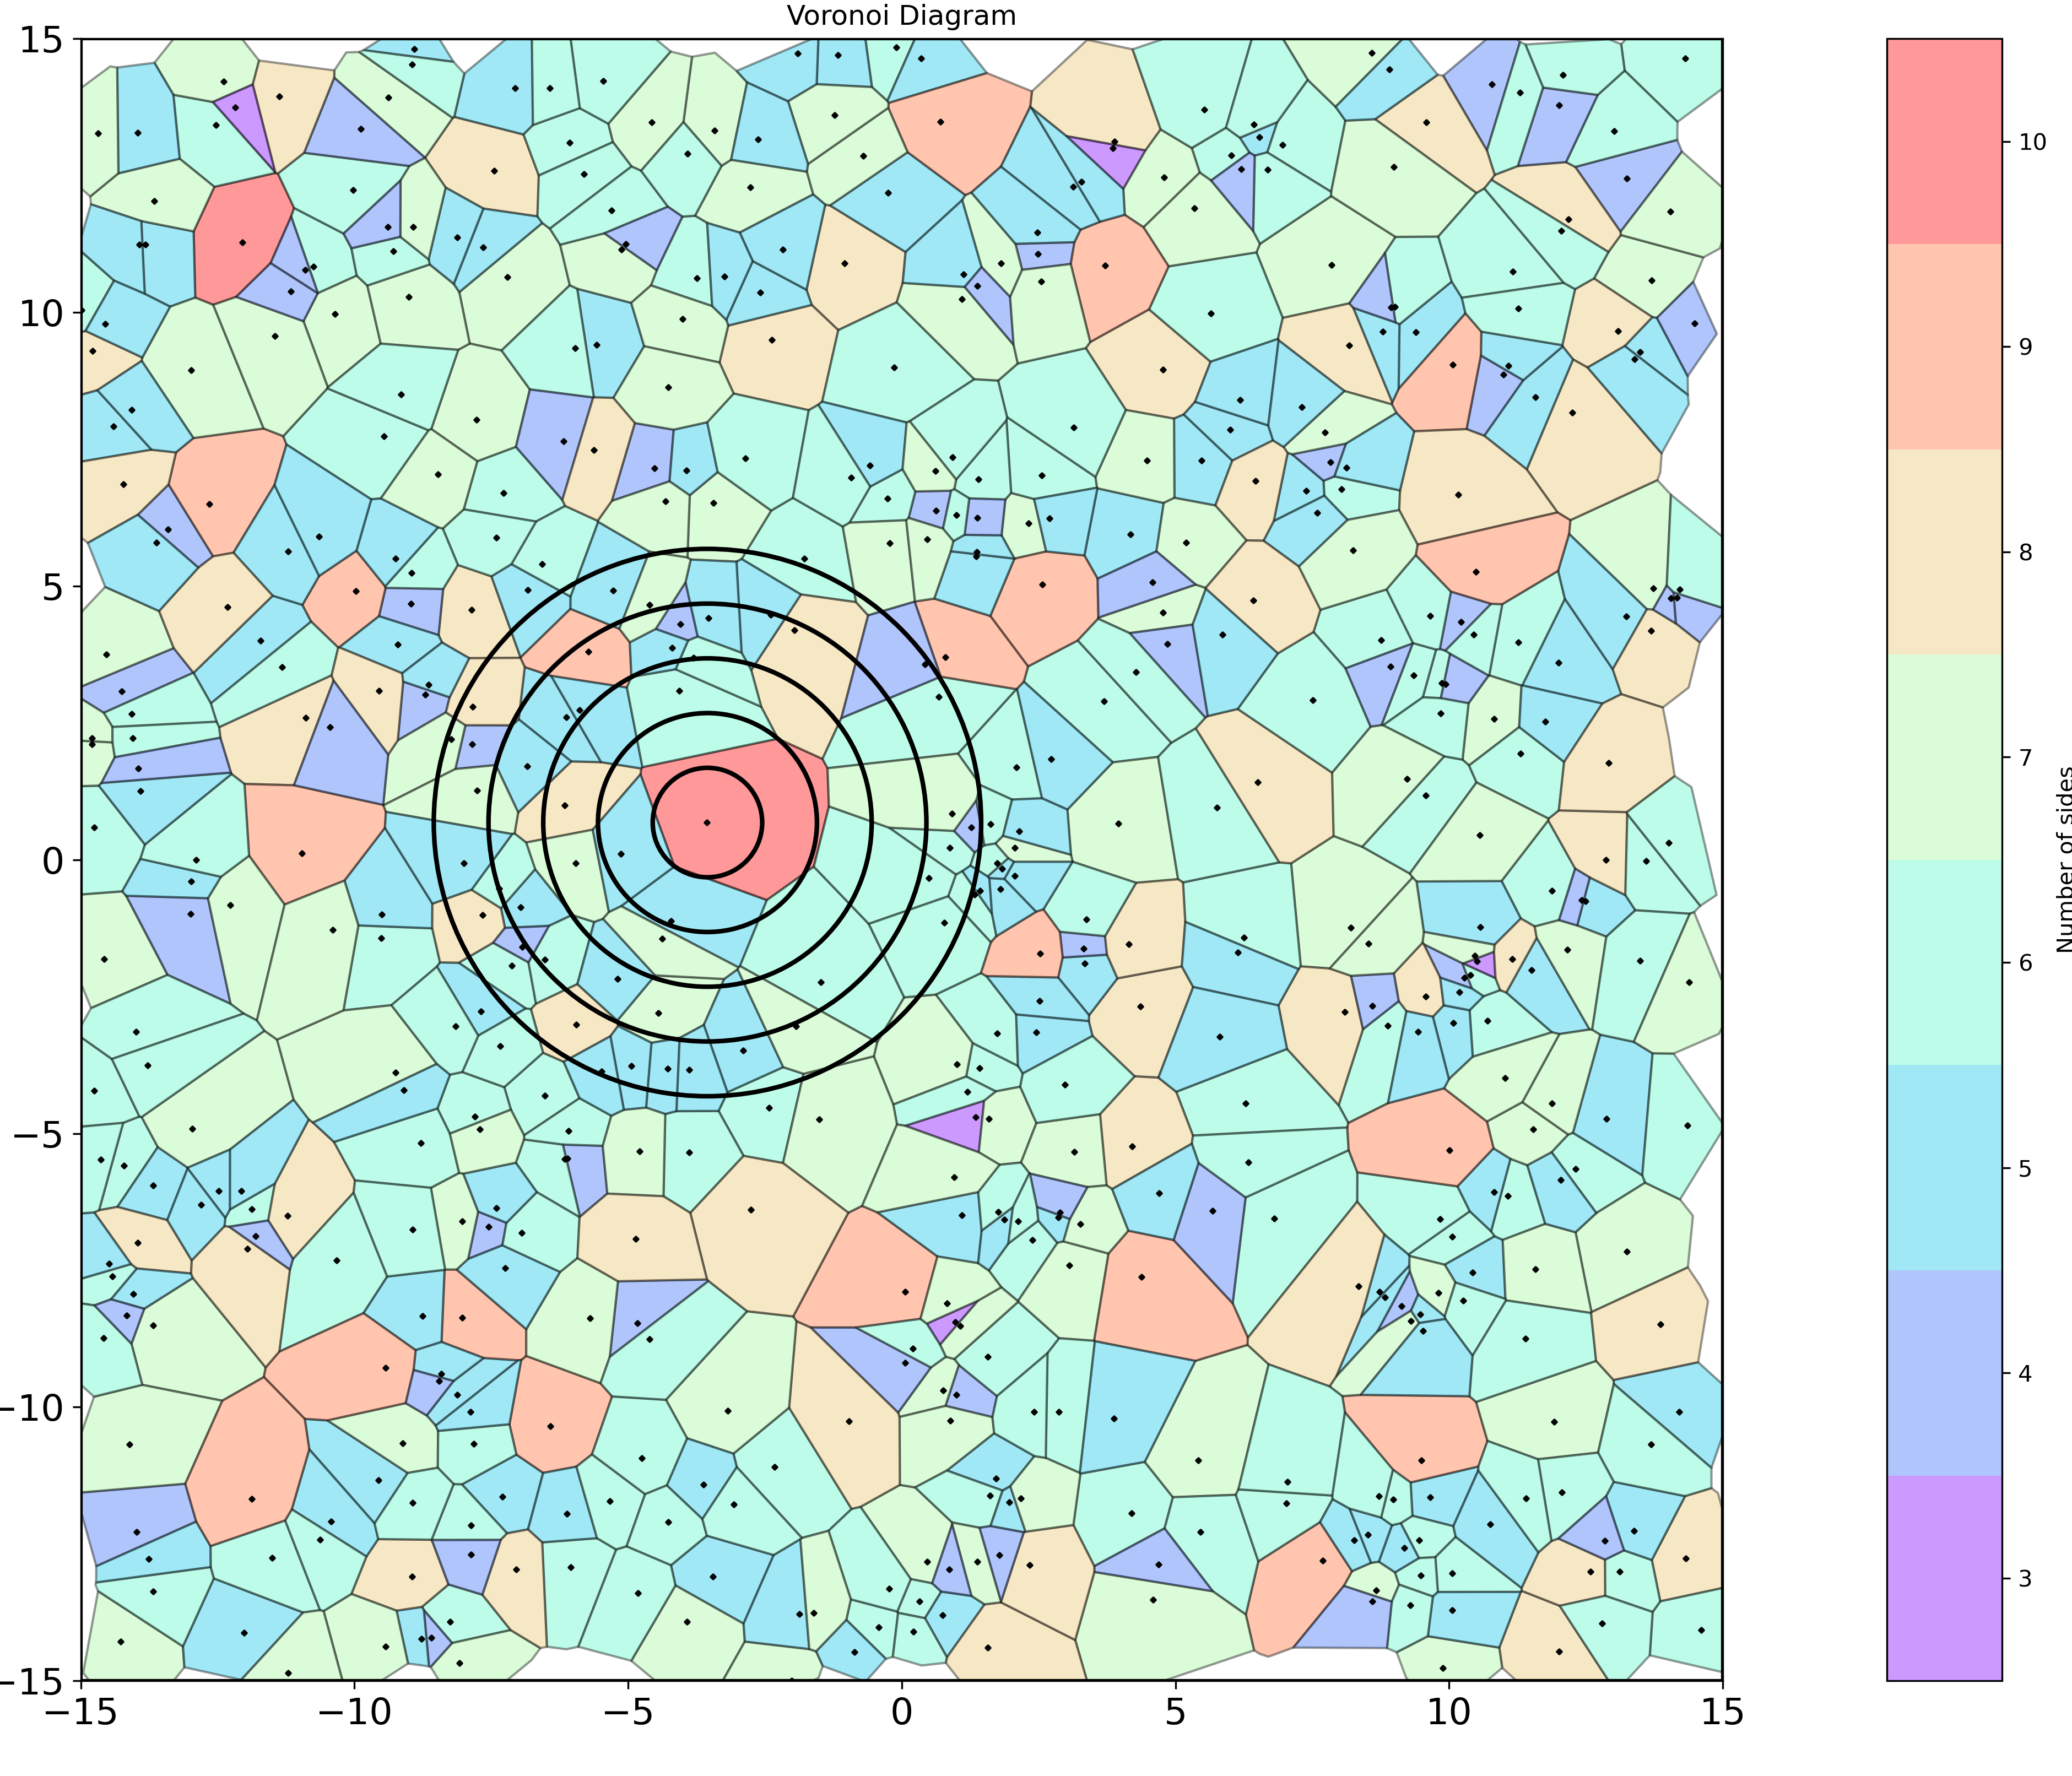
\includegraphics[width=\linewidth]{figures/crystalline_voronoi_d_cut_circles.png} 
    \caption{Zoomed section of \autoref{fig:2d} wherein we see a cartoonized version of a dcut radius cutoff
    used to suppliment Voronoi analysis. Circles represent the neighbor cutoff
    radius(dcut) beyond which we truncate chromophores from the neighborlist.
    Cells are colored by number of neighbors.}
  \label{fig:dcut}
\end{figure}

However, artifact of constructing nieghborlists in this way is that some
neighbors are too far apart to interact electronically, but are nevertheless closer to each other than they
are to any other chromophores and are therefore counted as neighbors. 
Inspection of \autoref{fig:dcut} reveals how this phenomena can arise from this type of construction.
Because charges will not hop between these pairs, including them in the pair list will result in 
superfluous QCCs. 

In light of this, we introduce a parameter by which we further pare down the neighbor list. This parameter is
a naive cutoff distance, referred to as `dcut' in this thesis. We visualize various dcut values as black
circles in \autoref{fig:dcut}.
It is clear from this image that the choice of dcut is could drastically effect the
neighborlist.  
Note that the z-direction has been collapsed, and the distances do not necessarily correlate to the distance
between chromophores in the system.

A proper choice of dcut will depend on the material under investigation, 
as the size of the individual chromophores will vary. In 
\autoref{dcutresults}, we test the sensitiviy of our results to the value of dcut for the crystalline P3HT
data. From this testing, we consider if the juice is worth dcut's radial squeeze from a computational standpoint. 

\section{Kinetic Monte Carlo}
\label{KMC}

With the MD data generated, the data chopped into individual chromophores, 
the chromophores and chromophore pair energetics
quantified with QCC, and the Marcus hop rate calculated, 
a single charges movement through the morphology can be simulatied with the
application of a KMC algorthim.

Monte Carlo algorithms use pseudorandom numbers to solve computational problems. Our implementation can be
described as a first choice method KMC algorithm, where the kinetics involved is the rate of one electron
charge transfer reactions and the first choice is that of the fastest available hop for a given charge.

Using MorphCT, a charge is implanted as quasi-particle into a random chromophore within 
the morphology. In this model, we assume that the only events that can take place in the system are hops
between chromophores. With this, the rate of all possible events in the system are known and are given by
\autoref{marcus}. 

With the charge implanted, the hop rate, $k_{ij}$, from the occupied chromophore to any
given neighboring chromophore is taken to be
inversely proportional to the amount of time, $\tau$, that the system will have to wait before that hop will
take place. The $\tau$ of all available hops forms a queue of hops from shortest wait time, fastest hop, to
longest wait time, slowest hop. From this queue, the shortest wait time (first choice) can be selected
and the system can be moved forward in time by $\tau$.

However, hopping processes at the angstrom level do not proceed deterministically. 
Our implementation, and others like it [NEED REFS?], have
successfully captured the stochasticiity of these systems via a shuffling our hopping queue.
The shuffled wait time for every potential hop from occupied chromophore $i$ onto a
neighboring chromophore $j$ looks as follows:

\begin{align}
    \tau = \frac{1}{k_{ij}} \cdot \ln{\frac{1}{x}} 
\end{align}
where x is a random number between 0 and 1 and $\log{(1/x)}$ is a scaling factor. To illucidate this
graphically, $\ln{(1/x)}$ is plotted in figure \ref{fig:ln} from 0 to 1. From this we can see that with
a large enough sampling, significant reshuffling of the queue will take place, allowing for a rare hop to jump
the queue.

\begin{figure}
  \center
  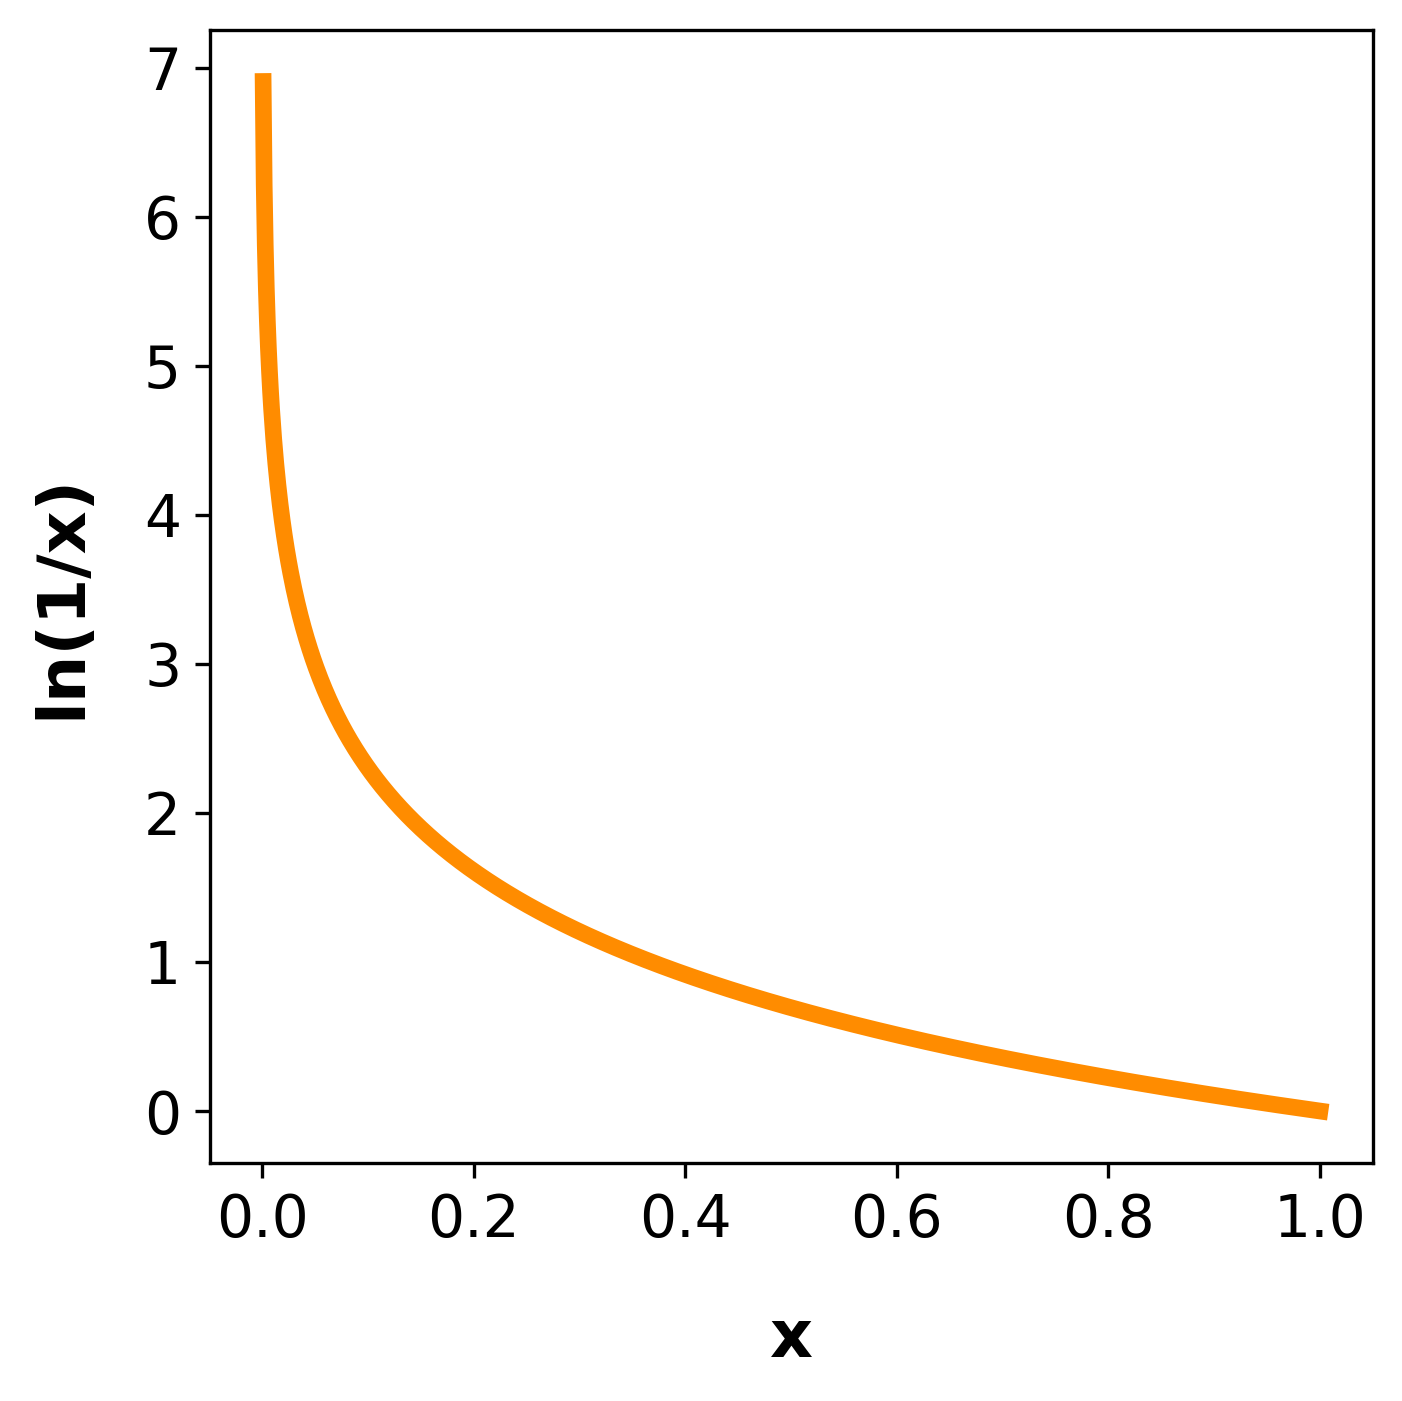
\includegraphics[width=0.8\linewidth]{figures/naturallog.png}
  \caption{Graphical insight into the reshuffling of the wait time queue. Here the x-axis represents the 
    interval from which numbers are drawn randomly such that the wait times in the queue can be scaled 
    by ln(1/x).}
  \label{fig:ln}
\end{figure}

From the rationally shuffled queue, the shortest waittime is chosen and the charge is moved to
its new chromophore host. The system is then considered to have moved forward in time by $\tau$. This proceeds
until the charge carrier stalls out or hops past a prespecified lifetime. How we aggregate data from 1000's of
single KMC simulations to obtatin macroscopic charge mobility is the subject of the following section.



\subsection{KMC analysis}

MorphCT allows for the creation of a system object that holds all the information necesarry to carry out the
KMC simulations outlined above. Running the simulation requires the choice of three system parameters: the
KMC temperature, the carrier liftimes, and the number of indivual KMC simulations to perform.

The choice of carrier lifetimes effectively serve as checkpoints at which the displacement of charge carriers is recorded. For
each specified lifetime, the prescribed number of individual KMC simulations is run as described above. When a
given charge carrier hops past the specified lifetime, that is, the addition of the current iterations $\tau$ advances
the simulation beyond the specified lifetime, 
its displacement from its starting location is stored in the carrier object. After repeating this over a
statistically significant number of carriers, the carrier data can be aggregated and the mean squared
displacement (MSD) for particles over that amount of time can be calculated. MSD over a given time period is 
the standard deviation in position for a charge walking randomly through this electronic environment. 

It is known that the MSD of a diffusive particle increases linearly as time goes to infinity. 
The slope of the MSD, $D$, as time
goes to inifinity can be estimated as a linear fit between the MSD's at the specified lifetimes.

There is no objective best practice for determing the slope of the MSD as
time goes to inifinty from simulation data of this kind \cite{Maginn2018}. With that, we seek primarily to simplifiy the MSD analysis as much as
possible so as to accuratley report this stage of the analysis for clarity but also to facilitate apples to
apples comparisons to future works using this workflow. 

Finally, the results of the MSD analysis are then used to determine the zero-field mobility using the following Einstein-Smoluchowski relation:

\begin{align}
    \label{einstein}
    \mu_{0} = \frac{eD}{6k_{B}T},
\end{align}

where $e$ is the elemental charge of a charge carrier, $D$ is the diffusion coefficient, $k_{B}$ is Planck's
constant and $T$ is temperature.  

A benifit to Monte Carlo analysis of this type is that charge carriers can be simultaneously. It is considered
to be "embarrasingly parrel," in that the subprocesses(charge carriers) require no communication.
MorphCT utilizes the python multiprocessing module to divide the prescribed number of charge carriers to be
simulated accross all available cores.

MorphCT takes GSD files which are
the native file format of the simulation engine HOOMD-blue \cite{Anderson2020a} which is the scaffolding of
Planckton.
%%% Local Variables: 
%%% mode: latex
%%% TeX-master: "BSUmain"
%%% End: 
